% --------------------------------------------------------------------------- %
\subsection{Диаграммы потоков данных}
% --------------------------------------------------------------------------- %
\begin{frame}
    Описание алгоритма -- ориентированный граф. В его вершинах -- процессы обработки данных, рёбра -- пути данных между процессами.

    \begin{figure}
        \centering
        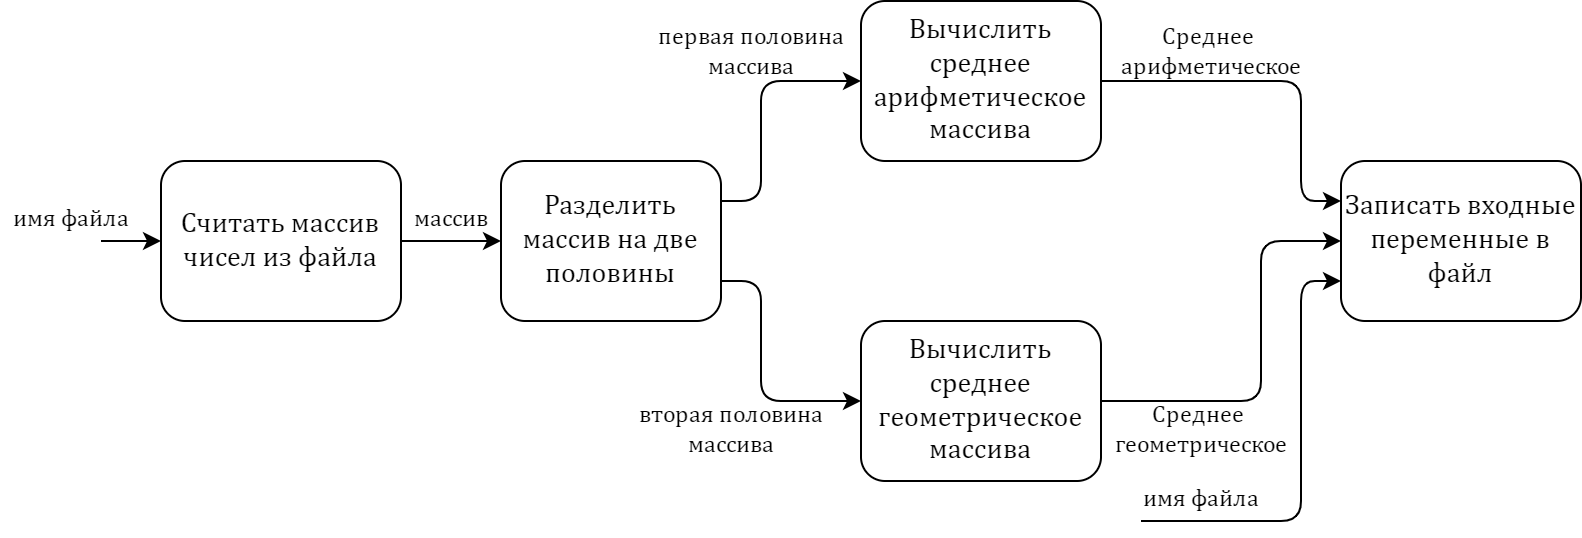
\includegraphics[width=0.8\textwidth]{images/illustration.dataflow.png}
        \caption{Пример диаграммы потоков данных, описывающей вычисление среднего арифметического и среднего геометрического двух половин массива целых чисел с последующей записью результатов в файл}
    \end{figure}

\end{frame}


\subsection{pSeven -- реализация диаграмм потоков данных}
%%%%%%%%%%%%%%%%%%%%%%%%%%%%%%%%%%%%%%%%%%%
\begin{frame}
    \begin{figure}
        \centering
        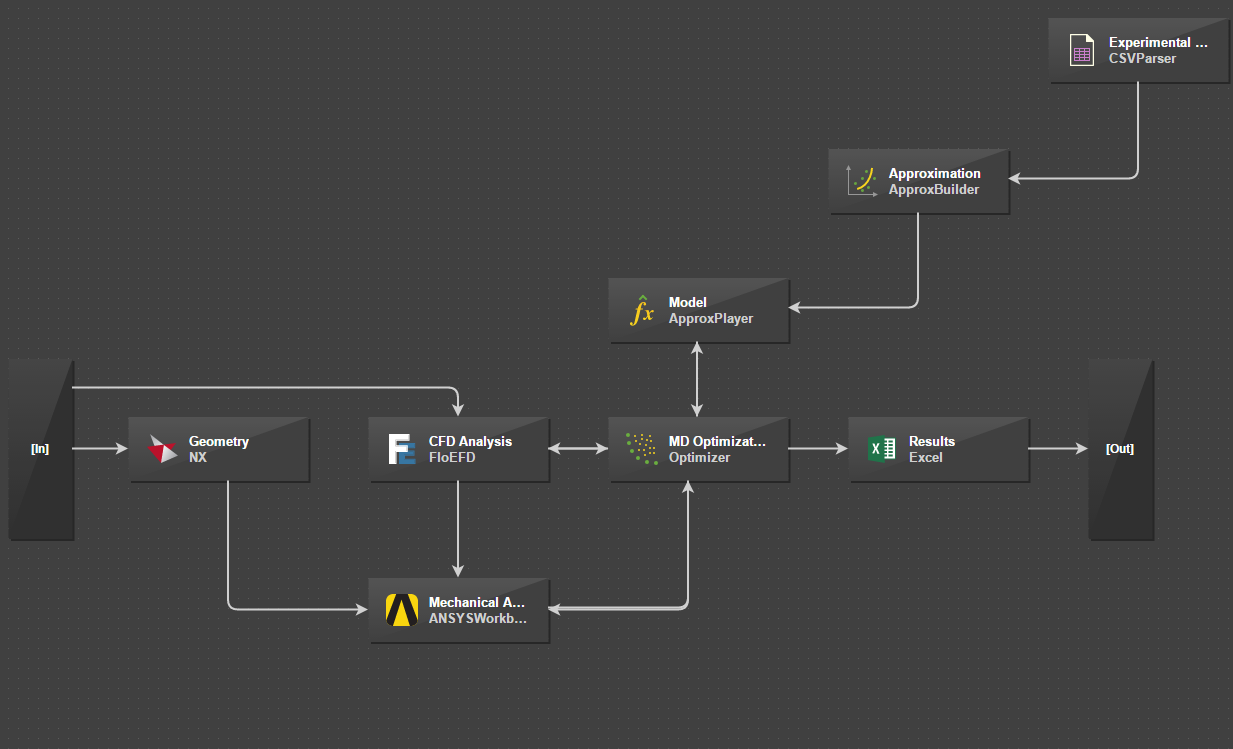
\includegraphics[width=\textwidth]{images/workflow1.png}
        \caption{Графический пользовательский интерфейс pSeven}
    \end{figure}

\end{frame}

% --------------------------------------------------------------------------- %
\subsection{Результаты сравнения. Выявленные достоинства объекта разработки}
% --------------------------------------------------------------------------- %
\begin{frame}
    Основные достоинства comsdk по сравнению с pSeven:
    \begin{itemize}
        \item Нет необходимости указывать входные и выходные данные при описании алгоритма.
        \item По умолчанию поддерживаются алгоритмы, подразумевающие взаимодействие с пользователем
    \end{itemize}

    \begin{figure}
        \centering
        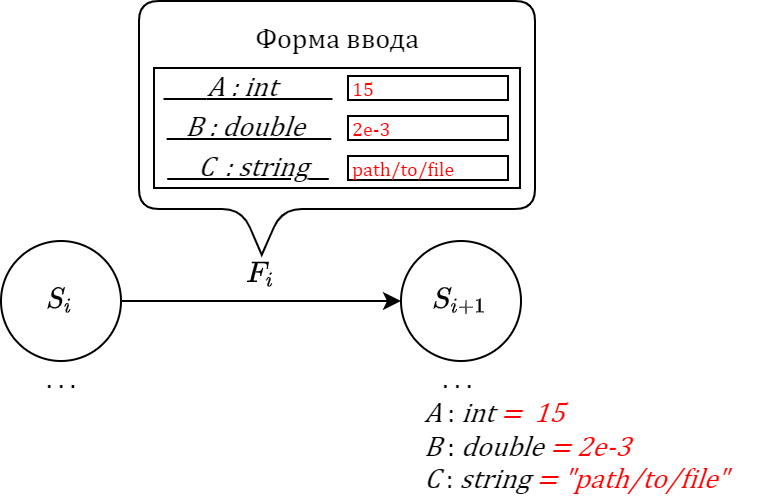
\includegraphics[height=0.33\textheight]{images/illustration.form_generation.png}
    \end{figure}

    \begin{itemize}
        \item Результат применения -- компилируемая программа с возможностью запуска на различных платформах.
    \end{itemize}
\end{frame}

% --------------------------------------------------------------------------- %
\subsection{Результаты сравнения. Выявленные недостатки объекта разработки}
% --------------------------------------------------------------------------- %
\begin{frame}
    Основные недостатки comsdk по сравнению с pSeven:
    \begin{itemize}
        \item Отсутствие поддержки матричных типов данных.
        \item Отсутствие средств визуализации результатов расчётов.
        \item Отсутствие возможности использования при расчётах распределённых вычислительных систем;
    \end{itemize}
\end{frame}
%%%%%%%%%%%%%%%%%%%%%%%%%%%%%%%%%%%%%%%%%%%